\documentclass[a4paper,12pt]{article}
 \usepackage{graphicx}
 \usepackage{fancyhdr}
 \usepackage{url}
 \usepackage{subfigure}
 \usepackage{geometry}
 \usepackage{caption}
 \usepackage{multirow}
\usepackage{amsmath,amssymb}
\usepackage{CJK}
\usepackage{diagbox}
\usepackage{graphicx}
\usepackage{geometry}
\usepackage{amsfonts}
\usepackage{indentfirst}
%\usepackage{type1cm}
\usepackage{bm}
\usepackage{amsmath}
\usepackage{amssymb}
\usepackage{minted} 
%\usepackage{algorithm} %format of the algorithm %sao
%\usepackage{algorithmic} %format of the algorithm %sao
%\usepackage[ruled]{algorithm2e}%sao
\usepackage{tcolorbox}
\usepackage{multirow} %multirow for format of table
%\usepackage{xcolor}
\usepackage{color}
%\usepackage{epstopdf}
\usepackage{enumerate}
\usepackage{graphicx}
\usepackage{subfigure}
\usepackage{float}
\pagestyle{fancy}
 \title{
\includegraphics[scale=1.44]{biaoti.png}\\
\vspace{0.3cm} \hrule
\vspace{3cm}\huge{{\bf VE401 Term Project 1}}\\ \vspace{1.2cm} \huge{Pseudo-random Numbers}\vspace{1.5cm}}


\author{
\begin{tabular}{ll}
Hu Zhengdong & 517370910249\\
Wang Yisen & 517370910202\\
Xu Mengjing &517370910042\\
Zhang Hexin & 517370910134\\
Zou Jiayun & 517370910191\\\\\\\\\\
\end{tabular}}

\begin{document}
 	\maketitle
 	\newpage

	\section*{Abstract}
\noindent In this project, we look into pseudo-random numbers and highlight the test of the randomness of pseudo-random numbers. To gather information, we first generate a sequence of pseudo-random numbers. Then we apply all together three tests: the frequency test (or monobit test), the Wald-Wolfowitz runs test and the frequency test within a block [4]. The first test is the basic of the other tests. The second test is more reliable while problems still exist. Therefore, we also search a third test to give more evidence. With these three tests, we develop a general procedure of randomness checking. Moreover, we can safely come to a conclusion that we have no evidence against the randomness of the sequence of pseudo-random numbers we generate.\newpage
 	\tableofcontents
 	\newpage
	\section{Introduction}
\noindent Pseudo-random numbers are a sequence of random-looking numbers that is not actually random, but looks random, in a way that people can not easily tell the subsequent numbers given the first few numbers [6]. To know more about the pseudo-random numbers, we first need to learn about the birth of random numbers. A classic example of generating random numbers is the dice, the oddest of which was discovered in a 24th century B.C. in the Middle East [8].\\\\
\centerline{\includegraphics[scale=0.4]{dice.png}}
\centerline{Figure 1. Ancient six-sided dice [8]}
\noindent \\\\ After thousands of years, in the mid 1940s, with the increasing demand of random numbers for researches, a corporation called RAND was first able to generate a sequence of high-quality random numbers using a machine. In 1951, the instruction for generating random numbers finally existed in a real computer [8].\\

\noindent However, random numbers are so random that they provide many uncertainties and inconveniences for programmers at that time. Therefore, John von Neumann came out an idea of developing a so-called pseudo-random numbers. His idea is  using a deterministic math function with the same initial conditions to generate numbers. It is the origin of pseudo-random numbers. Although his method has some problems, it is still a breakthrough [8].\\\\
\centerline{\includegraphics[scale=0.5]{von.png}}
\centerline{Figure 2. John von Neumann (1903-1957) [9]}
\noindent \\\\After that, the pseudo-random numbers generator has been developed, and thus we have more ways to generate a sequence of pseudo-random numbers. People today still dispute over which method is the best [8]. \\

\noindent From the development of random numbers and pseudo-random numbers, we know that the research of pseudo-random numbers is indeed necessary. The main difference between pseudo-random numbers and random numbers is that random numbers are usually generated naturally like throwing dice and decay of a radioactive element, while pseudo-random numbers are usually generated by software functions. But pseudo-random numbers have many advantages over random numbers in that they are very useful for debugging and simulation. It reduces the running time and avoids uncertainties [7].\\


\noindent In this project, we will apply three tests to judge the randomness of pseudo-random numbers. We would like to first provide a brief introduction to these three tests.
\subsection{Frequency Test}
\noindent The focus of the frequency test is the proportion of zeroes and ones for the entire sequence. The purpose of this test is to determine whether the number of ones and zeros in a sequence are approximately the same as would be expected for a truly random sequence. The test assesses the closeness of the fraction of ones to $\frac{1}{2}$, that is, the number of ones and zeroes in a sequence should be about the same. All subsequent tests depend on the passing of this test. [4]
\subsection{Wald-Wolfowitz Runs Test}
 \noindent The Wald-Wolfowitz runs test, which is also known simply as runs test, can be used to check a null hypothesis for a data sequence which only contains two different values. It can be used to test whether the elements in a certain sequence are mutually independent and identically distributed instead of whether they have equal probabilities of occurring. A run of a sequence is a maximal non-empty block in a sequence which consists of adjacent equal elements. By finding the actual number for runs, we can calculate the probability of gaining this number of runs. Since the calculation is tedious, we can use the binomial distribution to approximate it. After we find the probability, we can decide whether to reject the null hypothesis that this data sequence is random. [4]


\subsection{Frequency Test within a Block}
\noindent The frequency test within a block is first based on the frequency test. The main difference lies in that this test focus on the frequency rather than the simple proportion of the sample. The frequency test within a block is also regarded the most reliable and detailed among all the three tests. It defines a blockFrequency ($M$, $n$) where $M$ is the length of each block and $n$ is the length of the bit string. Its purpose is to determine whether the frequency of ones in an M-bit block is about $M/2$. After computing the $P$-value of the test, if it is too small, we would reject the randomness of the pseudo-random numbers and accept it otherwise.
\section{Generating Random Bit-String}
\noindent In this project, we will use the language C++ and the compiler {\emph Clion} to generate our random bit-string. Plus, we will also use C++ to perform some complicated calculations in section 3. The code for generating our bit-string in Appendix 7.1. \\
%zjykeyword %sao
%\begin{tcolorbox}[title = {Code for generating our bit-string}]
%\begin{minted}{c++}
%#include <iostream>
%#include <iomanip>
%#include <sstream>
%#include <fstream>
%using namespace std;
%int main() {
%srand((unsigned)time(NULL));
%ofstream oFile;
%oFile.open("random.txt");
%int one, zero;
%one = 0;
%zero = 0;
%for (int i = 0; i < 500; i++)
%{
%    int a = rand()%2;
%    if (a == 1) one++;
%    else zero++;
%    oFile<<a;
%}
%oFile<<endl;
%cout<<"number of 1s: "<<one<<endl;
%cout<<"number of 0s: "<<zero<<endl;
%oFile<<"number of 1s: "<<one<<endl;
%oFile<<"number of 0s: "<<zero<<endl;
%oFile.close();
%return 0;
%}
%\end{minted}
%\end{tcolorbox}
\noindent We use an output file "random.txt" to store our datum:\\
\begin{tcolorbox}[title = {random.txt}] %sao
11001101010001100000100100100001100011101011100010010011100100010\\10000100011010001011110101010110011101011100000110111110001100111\\01100001001001001010010001110011011111111001100110000011000011000\\00110110101110010010010110000001000111101110101010111010111100001\\00011011110011111000100011000110010101100101111111010001000110111\\10100100001011111001101000101001011110001000100101001101110000110\\00100101011011101010110101010101010111111010001010110010110010010\\111001010110000101010000110110110011111001101\\
number of 1s: 246\\
number of 0s: 254
\end{tcolorbox}

\noindent Please note that we will use this particular bit-string throughout the entire section 3. Furthermore, we will apply all three tests mentioned above to this particular bit-string so as to check if C++ can generate high-quality random numbers.

\section{Tests on Randomness}
\subsection{Frequency Test}
\noindent We suppose a random number generator produces a bit sequence ($b_n$) of values $b_n = 0$ or $b_n = 1$. We denote this random variable by $B_n$, with a probability of 1/2, either 0 or
1. To check for randomness, it is often convenient to transform this sequence to values $x_n = 2b_n -1$, so that $x_n = -1$ or $x_n = +1$. Now suppose that $X_n$ is the random variable that produces, and $X_n$ satisfies that $X_n=2B_n-1$. Another random variable constructed is $Y_n$, which is the sum of the values $B_n$. The frequency test or monobit test is based on summing up the values $X_n$, which produces the random variable $S_n$. We will explore the use of $\left|S_{n}\right| / \sqrt{n}$ in the frequency test in this part.
\subsubsection{Property of $\left|S_{n}\right| / \sqrt{n}$}
\noindent  To find out the distribution of $\left|S_{n}\right| / \sqrt{n}$, we first need to focus on $Y_n$, which is a binomial distribution with the probability of success $p$=$\frac{1}{2}$ and the number of trials $n$, and $B_n$ is the corresponding Bernoulli distribution. The relation between $Y_n$ and $B_n$ is shown below.
\begin{equation}
Y_n=B_1+B_2+\cdots+B_n
\end{equation}
Since $p$ is $\frac{1}{2}$ and $n$ can be very large, we can use the normal distribution to approximate $Y_n$.
\begin{equation*}
\begin{split}
\mu_y&=np=\frac{1}{2}n\\
\sigma_y^2&=npq=\frac{1}{4}n
\end{split}
\end{equation*}
\noindent Then the approximation is
\begin{equation}
f_Y(x)\approx \frac{1}{\sqrt{2\pi}\sqrt{npq}}e^{\frac{-(x-np)^2}{2npq}}
\end{equation}

\noindent Since $X_n=2B_n-1$, we can connect $Y_n$ with $S_n$.
\begin{equation}
\begin{split}
S_n&=X_1+X_2+\cdots+X_n\\
   &=(2B_1-1)+(2B_2-1)+\cdots+(2B_n-1)\\
   &=2(B_1+B_2+\cdots+B_n)-n\\
   &=2Y_n-n
\end{split}
\end{equation}
By the property of the normal distribution, $\frac{S_n}{\sqrt{n}}$ can also be approximated as a normal distribution with the mean and variance changed.

\begin{equation*}
\begin{split}
u_{\frac{S_n}{\sqrt{n}}}&=\frac{2u_y-n}{\sqrt{n}}=0\\
\sigma_{\frac{S_n}{\sqrt{n}}}^2&=\frac{4}{n}\sigma_y^2=1
\end{split}
\end{equation*}
\noindent The probability function of $\frac{S_n}{\sqrt{n}}$ is
\begin{equation}
f_{\frac{S_n}{\sqrt{n}}}(x)=\frac{1}{\sqrt{2\pi}}e^{-\frac{x^2}{2}}
\end{equation}
\noindent Then $\frac{S_n}{\sqrt{n}}$ is the standard normal distribution. The definition of half-normal distribution states that let X follow an ordinary normal distribution $N(0,\sigma ^{2})$, then $Y=|X|$ follows a half-normal distribution [1]. From the definition, we can conclude that $|\frac{S_n}{\sqrt{n}}|=\frac{|S_n|}{\sqrt{n}}$ is the half-normal distribution $|Z|$.\\

\noindent We can find the the density function of the half-normal distribution

\noindent For $z\geq 0$
\begin{equation}
\begin{split}
F_{|Z|}(z)&=P[|Z|\leq z]\\
		  &=P[-z\leq Z \leq z]\\
		  &=\frac{1}{\sqrt{2\pi}}\int_{-z}^{z}e^{-\frac{x^2}{2}}dx
\end{split}
\end{equation}
\noindent Then we differentiate the cumulative distribution function to get the density function.
\begin{equation}
f_{|Z|}(z)=F'_{|Z|}(z)=\sqrt{\frac{2}{\pi}}e^{-\frac{z^2}{2}}
\end{equation}

\noindent For $z<0$, $f_{|Z|}(z)=0$. Then
\begin{equation}
 	f_{|Z|}(z)=
 	\left\{
 	\begin{aligned}
	 &\sqrt{\frac{2}{\pi}}e^{-\frac{z^2}{2}} &,  z\geq 0 \\
	 &0&,  z < 0
 	\end{aligned}
 	\right.
 	\end{equation}

\noindent Then we can get the plot of the half-normal distribution.\\
\begin{figure}[htb]
\centering
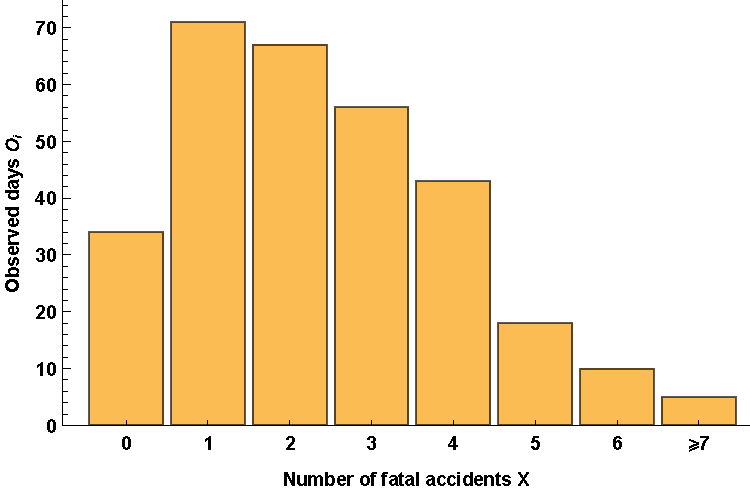
\includegraphics[scale=0.8]{1.png}
\end{figure}

\centerline{Figure 3. Half-normal distribution}
\subsubsection{Applying Frequency Test to Our Pseudo-Random Numbers}
\noindent We use the list of 500 pseudo-random 0s and 1s generated in section 2 in this part. The list is shown below.
\begin{tcolorbox}[title = {random.txt}] %sao
11001101010001100000100100100001100011101011100010010011100100010\\10000100011010001011110101010110011101011100000110111110001100111\\01100001001001001010010001110011011111111001100110000011000011000\\00110110101110010010010110000001000111101110101010111010111100001\\00011011110011111000100011000110010101100101111111010001000110111\\10100100001011111001101000101001011110001000100101001101110000110\\00100101011011101010110101010101010111111010001010110010110010010\\111001010110000101010000110110110011111001101\\
number of 1s: 246\\
number of 0s: 254
\end{tcolorbox}
\noindent which contains 246 1s and 254 0s.
\begin{equation*}
\begin{split}
\frac{|S_n|}{\sqrt{n}}&=\frac{|246-254|}{\sqrt{500}}\\
					  &=0.3578\\
P[|Z|\geq \frac{|S_n|}{\sqrt{n}}]&=\int_{0.3578}^{\infty}\sqrt{\frac{2}{\pi}}e^{-\frac{x^2}{2}}dx\\
                                 &=0.7204
\end{split}
\end{equation*}

\noindent  We can take the value as the $P$-Value of the null hypothesis that the generated numbers are random.  Since $0.7204>>0.01$ [4], we can't reject the null hypothesis. We will just accept that the generated sequence is random.\\

\subsection{Wald-Wolfowitz Runs Test}
\noindent We will first explain the concept of a run. A run of a sequence is a maximal non-empty block in a sequence which consists of adjacent equal elements. For instance, in 1110010, there are four runs. The first run is 111, the second is 00, the third is 1, the fourth is 0. We first set the null hypothesis that each element in the sequence is independent. Under this hypothesis, the number of runs in a sequence of n elements is a random variable which we denote as $R$. And we denote the random variable for the number of runs of 0 to be $R_1$, the random variable for the number of runs of 1 to be $R_2$. We denote $n_1$ to be the actual number of runs of 0, and $n_2$ to be the actual number of runs of 1. $n$ is the total number. That is to say, $n = n_1+n_2$.
\subsubsection{The Range and Mean of the Wald-Wolfowitz Runs Test}
\noindent We determine the range of R first. Suppose $R_1$ is the number of runs of 1s and $R_2$ is the number of runs of 0s.

\noindent Since  $n_1\neq 0$ and $n_2\neq 0$, there is at least one run of 1s and one run of 0s.
\begin{center}
$R_1\geq 1$ , $R_2\geq 1$, $R=R_1+R_2\geq 2$
\end{center}

\noindent if $n_1>n_2$, all the 0s can be completely separated from each other by 1s, on which condition $R_1$ and $R_2$ can attain the maximum at the same time.
\begin{center}
$R_1\leq n_2+1$, $R_2\leq n_2$, $R=R_1+R_2\leq 2n_2+1=2$min$(n_1,n_2)+1$
\end{center}
\noindent if $n_1=n_2$, the 0s and 1s can both be completely separated from each other at the same time.
\begin{center}
$R_1\leq n_1$, $R_2\leq n_2$, $R=R_1+R_2\leq n1+n_2\leq 2$min$(n_1,n_2)$
\end{center}
\noindent if $n_1\geq n_2$, all the 1s can be completely separated from each other by 0s, on which condition $R_1$ and $R_2$ can attain the maximum at the same time.
\begin{center}
$R_1\leq n_1$, $R_2\leq n_2+1$, $R=R_1+R_2\leq 2n_1+1=2$min$(n_1,n_2)+1$
\end{center}
\noindent So the range of R is
\begin{center}
$2\leq R\leq 2$min$(n_1,n_2)+1$
\end{center}
Then we can determine the expectation of $R$p [2]. The first number of the sequence can be counted as one run, and the rest of the numbers can be counted as one run only when it is different from the previous number indicated by $I_j$. If $I_j=1$, it means that the number begins a new run. If $I_j=0$, it means that the number is included in the previous run. Then we can represent the number of runs R as
\begin{equation}\label{3.2.1.1}
R=1+\sum_2^{n_1+n_2}I_j
\end{equation}
\noindent Then we can find the expectation of $R$.
\begin{equation}
\begin{split}
E[R]&=E[1+\sum_2^{n_1+n_2}I_j]\\
	&=E[1]+E[\sum_2^{n_1+n_2}I_j]\\
	&=1+E[\sum_2^{n_1+n_2}I_j]
\end{split}
\end{equation}

\noindent We can take $I_j$ as a Bernoulli random variable with the probability of success p.
\begin{equation}
\begin{split}
p&=\frac{n_1}{n_1+n_2}\frac{n_2}{n_1+n_2-1}+\frac{n_2}{n_1+n_2}\frac{n_1}{n_1+n_2-1}\\
&=\frac{2n_1n_2}{(n_1+n_2)(n_1+n_2-1)}
\end{split}
\end{equation}

\noindent Then we can insert the probability into the expectation of the sum of the Bernoulli random variables to find $E[\sum_2^{n_1+n_2}I_j]$.
\begin{equation}
\begin{split}
E[\sum_2^{n_1+n_2}I_j]&=(n_1+n_2-1)p\\
	&=(n_1+n_2)\frac{2n_1n_2}{(n_1+n_2)(n_1+n_2-1)}\\
	&=\frac{2n_1n_2}{n_1+n_2}\\
	&=\frac{2n_1n_2}{n}
\end{split}
\end{equation}
\noindent Then we can calculate the expectation of runs $E[R]$.
\begin{equation}
E[R]=1+E[\sum_2^{n_1+n_2}I_j]=1+\frac{2n_1n_2}{n}
\end{equation}
To conclude, we have proved that
\begin{center}
$2\leq R\leq 2$min$(n_1,n_2)+1$,\qquad $E[R]=\mu_R=\frac{2n_1n_2}{n}+1$;
\end{center}

\subsubsection{The Probability for $k$ being Even and Odd}
\noindent Suppose in a given sequence, there are $n_1$ 0-bits and $n_2$ 1-bits. The total number of bits is $n=n_1+n_2$.\\\\
According to Cardano's Principle, we know that the probability of $R=k$ is
\begin{equation*}
P[R=k]=\frac{\text{number of ways of getting } k \text{ runs}}{\text{total number of ways of arranging 0's and 1's}}
\end{equation*}
Let us first calculate the value of the denominator. There are $(n_1+n_2)$ 0's and 1's in total, and we can select $n_1$ places out of $(n_1+n_2)$ to put 0-bits. Once the positions of 0-bits are determined, the positions of 1-bits are also determined. Therefore, the denominator can be represented as
\begin{equation*}
\text{denominator}=\binom {n} {n_1}
\end{equation*}
Once we have calculated the denominator, let us deal with the nominator. Since we have proved in section 3.2.1 that the number of runs given $n_1$ and $n_2$ is within the following range,
\begin{equation*}
2\leq R \leq 2 \text{min}(n_1,n_2)+1
\end{equation*}
we can easily derive that when $R=2k'$ ($k'$ is a positive integer), $n_1$ 0-bits and $n_2$ 1-bits each account for $k'$ runs respectively. Similarly, when $R=2k'+1$, either $n_1$ 0-bits have $k'+1$ runs and $n_2$ 1-bits have $k'$ runs or $n_1$ 0-bits have $k'$ runs and $n_2$ 1-bits have $k'+1$ runs.\\\\
 Now, let us first consider the case when $R=k$ and $k=2k'$. Since there are $n_1-1$ spaces among 0-bits, if we want to divide 0-bits into $k'$ runs, we need to select $k'-1$ spaces. Therefore, the number of dividing $n_1$ 0-bits into $k'$ runs is \\
\begin{equation*}
\binom {n_1-1} {k'-1}
\end{equation*}
Similarly, the number of dividing $n_2$ 1-bits into $k'$ runs is
\begin{equation*}
\binom {n_2-1} {k'-1}
\end{equation*}
When we put $n_1$ 0-bits and $n_2$ 1-bits together, the runs of 0-bits and 1-bits should take turns. We can get the combination as [3]
\begin{equation*}
\binom {n_1-1} {k'-1} \binom {n_2-1} {k'-1}
\end{equation*}
Whether 0-bits start first or 1-bits start first gives different sequences, so we multiply the combination by 2, and we get the number of ways of getting $R=2k'$ runs.
\begin{equation*}
  2 \binom {n_1-1} {k'-1} \binom {n_2-1} {k'-1}
\end{equation*}
Therefore, by substituting $k'$ with $\frac{k}{2}$, we can derive the probability of $R=k$  when $k$ is even. [3]
\begin{equation}\label{3.2.2.1}
P[R=k]=\frac{2 \binom {n_1-1} {\frac{k}{2}-1} \binom {n_2-1} {\frac{k}{2}-1}}{\binom {n} {n_1}}
\end{equation}
When $R=k$ and $k=2k'+1$, if 0-bits have $k'+1$ runs, then we need to choose $k'$ spaces from $n_1-1$ spaces. The number of ways is presented by
\begin{equation*}
\binom {n_1-1} {k'}
\end{equation*}
Then 1-bits have $k'$ runs, so the number of ways to choose $k'-1$ spaces from $n_2-1$ spaces is
\begin{equation*}
\binom {n_2-1} {k'-1}
\end{equation*}
Therefore, when 0-bits have $k'+1$ runs and 1-bits have $k'$ runs, we have number of ways as [3]
\begin{equation*}
\binom {n_1-1} {k'} \binom {n_2-1} {k'-1}
\end{equation*}
Similarly, when 0-bits have $k'$ runs and 1-bits have $k'+1$ runs, we have number of ways as
\begin{equation*}
\binom {n_1-1} {k'-1} \binom {n_2-1} {k'}
\end{equation*}
The total number of ways of getting $2k'+1$ runs can be represented as
\begin{equation*}
\binom {n_1-1} {k'} \binom {n_2-1} {k'-1}+\binom {n_1-1} {k'-1} \binom {n_2-1} {k'}
\end{equation*}
Therefore, by substituting $k'$ with $\frac{k-1}{2}$, we can derive the probability of $R=k$  when $k$ is odd. [3]
\begin{equation}\label{3.2.2.2}
P[R=k]=\frac{\binom {n_1-1} {\frac{k-1}{2}} \binom {n_2-1} {\frac{k-1}{2}-1}+\binom {n_1-1} {\frac{k-1}{2}-1} \binom {n_2-1} {\frac{k-1}{2}}}{\binom {n} {n_1}}
\end{equation}
In summary, we have
\begin{equation}\label{as}
\begin{aligned}
P[R=k]&=\frac{2 \binom {n_1-1} {\frac{k}{2}-1} \binom {n_2-1} {\frac{k}{2}-1}}{\binom {n} {n_1}}, k\text{ is even}\\
P[R=k]&=\frac{\binom {n_1-1} {\frac{k-1}{2}} \binom {n_2-1} {\frac{k-1}{2}-1}+\binom {n_1-1} {\frac{k-1}{2}-1} \binom {n_2-1} {\frac{k-1}{2}}}{\binom {n} {n_1}},k\text{ is odd}\\
\end{aligned}
\end{equation}
\subsubsection{Example with Previously Generated 500 Pseudo-Random Numbers}
\noindent Using C++, we can find that the pseudo-random numbers sequence generated previously has 268 runs. Please refer to section 7.2 for the C++ code. The expectation of $R$ is: \\
\begin{equation*}
E[R]=1+\frac{2\times 254\times 246}{500}=250.936
\end{equation*}
Solving the inequality,
\begin{equation*}
|R-\mu _R|\geq |r-\mu_R|
\end{equation*}
we can find $R\geq 268$ or $R\leq 233$. Therefore,
\begin{equation*}
P[|R-\mu _R|\geq |r-\mu_R|]=1-P[234\leq R\leq 267]
\end{equation*}
We calculate the probability one by one with Excel by using eq. \eqref{as},
\begin{table}[H]\centering
\begin{tabular}{|c|c||c|c|}
\hline
$P[R=k]$ & $k$   & $P[R=k]$ & $k$   \\ \hline
0.01134               & 234 & 0.01289              & 235 \\ \hline
0.01464               & 236 & 0.01638              & 237 \\ \hline
0.01830               & 238 & 0.02015              & 239 \\ \hline
0.02216               & 240 & 0.02401              & 241 \\ \hline
0.02599               & 242 & 0.02770              & 243 \\ \hline
0.02951               & 244 & 0.03096              & 245 \\ \hline
0.03245               & 246 & 0.03350              & 247 \\ \hline
0.03456               & 248 & 0.03512              & 249 \\ \hline
0.03565               & 250 & 0.03565              & 251 \\ \hline
0.03561               & 252 & 0.03504              & 253 \\ \hline
0.03445               & 254 & 0.03337              & 255 \\ \hline
0.03228               & 256 & 0.03077              & 257 \\ \hline
0.02930               & 258 & 0.02748              & 259 \\ \hline
0.02575               & 260 & 0.02377              & 261 \\ \hline
0.02191               & 262 & 0.01991              & 263 \\ \hline
0.01806               & 264 & 0.01615              & 265 \\ \hline
0.01442               & 266 & 0.01268              & 267 \\ \hline
0.43637               &     & 0.43552              &     \\ \hline
\end{tabular}
\end{table}
\centerline{tpable 1. $P[R=k]$ for different value of $k$}
\noindent \\In which the last row represent the sums of the left column and the right column. Add them together, we have $P[234\leq R\leq 267] = 0.43637+0.43552 = 0.87189$.
\begin{equation*}
P[|R-\mu _R|\geq |r-\mu_R|]=1-P[234\leq R\leq 267] = 1- 0.87189 = 0.12811
\end{equation*}
The $P$- Value $0.12811>>0.01$ [4], so we cannot reject the null hypothesis that the generated numbers are random.\\\\
However, compare to the basic test, i.e. looking at the number of -1s and 1s, this run test gives us more insight.\\
\subsubsection{Approximate with Normal Distribution}
\noindent Since we have calculated $E[R]$ in the previous part, we can easily get the expression for $(E[R])^2$.\\
\begin{equation}\label{3.2.2.8}
(E[R])^2=(1+\frac{2n_1n_2}{n})^2=1+\frac{4n_1^2 n_2^2}{n^2}+\frac{4n_1n_2}{n}
\end{equation}
We can express $R^2$ in \eqref{3.2.2.3} using \eqref{3.2.1.1}
\begin{equation}\label{3.2.2.3}
\begin{aligned} R ^ { 2 } & = \left( 1 + \sum _ { j = 2 } ^ { n } I _ { j } \right) ^ { 2 } \\ & = 1 + \sum _ { j = 2 } ^ { n } I _ { j } + \sum _ { j = 2 } ^ { n } I _ { j } + \left( \sum _ { j = 2 } ^ {n} I _ { j } \right) ^ { 2 } \\  \end{aligned}
\end{equation}
According to the expression of $R$ in eq. \eqref{3.2.1.1}, we can further simplify $R^2$ as [2]
\begin{equation*}
\begin{aligned}
R^2 & = R + ( R - 1 ) + \left( \sum _ { j = 2 } ^ { n } I _ { j } \right) ^ { 2 } \\ & = 2 R - 1 + \sum _ { j = 2 } ^ { n } I _ { j } ^ { 2 } + \sum _ { j=2} ^ { n } \sum_{k=2,k\neq j}^{n} I _ { j } I _ { k }
\end{aligned}
\end{equation*}
We know that for certain pair of $(j,k)$ where $j=j'$ and $k=k'$, it gives $I_{j'}I_{k'}$. We will get the same value $I_{k'}I_{j'}$ where $j=k'$ and $k=j'$. Therefore,
\begin{equation*}
\begin{aligned}
R^2& = 2 R - 1 + \sum _ { j = 2 } ^ { n } I _ { j } ^ { 2 } + 2 \sum _ { j =2 } ^ { k-1 } \sum_{k=3}^{n} I _ { j } I _ { k }  \\
\end{aligned}
\end{equation*}
Because $I_j$ equals either 0 or 1, $I_j=I_j^2$.\\
\begin{equation*}
\begin{aligned}
R^2 &= 2 R - 1 + \sum _ { j = 2 } ^ { n } I _ { j } + 2 \sum _ { j=2 } ^ { k - 1 } \sum_{k=3}^{n} I _ { j } I _ { k } \\
 &= 2 R - 1 + ( R - 1 ) + 2 \sum _ { j=2 } ^ { k - 1 } \sum_{k=3}^{n} I _ { j } I _ { k }  \\
  &= 3 R - 2 + 2\sum _ { j < k } ^ {n } I _ { j } I _ { k }
\end{aligned}
\end{equation*}

\noindent Therefore, $E[R^2]$ can be calculated as
\begin{equation*}
\begin{aligned}
E \left[ R ^ { 2 } \right] & = E \left[ 3 R - 2 + 2 \sum _ { j < k } ^ { n } I _ { j } I _ { k } \right] \\ & = 3 E [ R ] - 2 + 2 E \left[ \sum _ { j < k } ^ { n } I _ { j } I _ { k } \right] \\  \end{aligned}
\end{equation*}
Since $I_j I_k$ either equals 0 or 1, we can substitute $E[I_j I_k]$ with $P(I_j I_k=1)$.
\begin{equation*}
\begin{aligned}
E[R^2]& = 3 \left( 1 + \frac { 2 n_1 n_2 } { n } \right) - 2 + 2 \sum _ { j < k } ^ { n } P \left( I _ { j } I _ { k } = 1 \right) \\ & = 1 + \frac { 6 n_1 n_2 } { n } + 2 \sum _ { j < k } ^ { n } P \left( I _ { j } = 1 , I _ { k } = 1 \right) \\
\end{aligned}
\end{equation*}
We can divide the sum into 2 cases. The first case is that $j$ and $k$ are adjacent(i.e. $k=j+1$) and $I_j = I_k=1$. The second case is that $j$ and $k$ are not adjacent and $I_j=I_k=1$. [2]
\begin{equation}\label{3.2.2.4}
\begin{aligned}
E[R^2] & = 1 + \frac { 6 n_1 n_2 } { n } + 2 \left( \sum _ { j = 2 } ^ { n-1 } P \left( I _ { j } = 1 , I _ { j + 1 } = 1 \right) + \sum _ { j = 2 } ^ { n-2 } \sum _ { k = j + 2 } ^ { n } P \left( I _ { j } = 1 , I _ { k } = 1 \right) \right) \\
&  = 1 + \frac { 6 n_1 n_2 } { b } + 2 \sum _ { j = 2 } ^ { n-1 } P \left( I _ { j } = 1 , I _ { j + 1 } = 1 \right) + 2 \sum _ { j = 2 } ^ {n-2 } \sum _ { k = j + 2 } ^ { n } P \left( I _ { j } = 1 , I _ { k } = 1 \right)  \end{aligned}
\end{equation}
In the first case, $I_j=I_{j+1}=1$. The $j$th number is different from the $(j-1)$th number  and the  $(j+1)$th number is different from the $j$th number. There are actually two sub-cases that satisfy this condition, namely 010 or 101. The probability of 010 is
\begin{equation*}
\frac { n_1 } { n } \cdot \frac { n_2 } { n - 1 } \cdot \frac { n_1 - 1 } { n - 2 }
\end{equation*}
Similarly, the probability of 101 is
\begin{equation*}
\frac { n_2 } { n } \cdot \frac { n_1 } { n - 1 } \cdot \frac { n_2 - 1 } { n - 2 }
\end{equation*}
Therefore, we can express 2 times the cumulative probability of the first case as follows. [2]
\begin{equation}\label{3.2.2.5}
\begin{aligned}
&2 \sum _ { j = 2 } ^ { n-1 } P \left( I _ { j } = 1 , I _ { j + 1 } = 1 \right)\\
&= 2  \sum _ { j = 2 } ^ { n-1 } \left[ \left( \frac { n_1 } { n } \cdot \frac { n_2 } { n - 1 } \cdot \frac { n_1 - 1 } { n - 2 } \right) + \left( \frac { n_2 } { n } \cdot \frac { n_1 } { n - 1 } \cdot \frac { n_2 - 1 } { n - 2 } \right) \right] \\  & =2  \sum _ { j = 2 } ^ { n-1 } \frac { n_1 n_2 ( n - 2 ) } { n  ( n - 1 ) ( n - 2 ) } \\
&=  \frac { 2 n_1 n_2 ( n - 2 ) } {  n  ( n - 1 ) }
\end{aligned}
\end{equation}
For the second case, since $j$ and $k$ are not adjacent, $P(I_j=1)$ is
\begin{equation*}
\frac { n_1 } { n } \cdot \frac { n_2 } { n - 1 }+\frac { n_2 } { n } \cdot \frac { n_1 } { n - 1 }=2 \cdot \frac { n_1 } { n } \cdot \frac { n_2 } { n - 1 }
\end{equation*}
Similarly, $P(I_k=1)$ can be calculated as
\begin{equation*}
 \frac { n_1 - 1 } { n - 2 } \cdot \frac { n_2 - 1 } { n - 3 }+ \frac { n_2 - 1 } { n - 2 } \cdot \frac { n_1 - 1 } { n - 3 }=2 \cdot \frac { n_1 - 1 } { n - 2 } \cdot \frac { n_2 - 1 } { n - 3 }
\end{equation*}
Since $P(I_j=1)$ and $P(I_k=1)$ are independent, $P \left( I _ { j } = 1 , I _ { k } = 1 \right)$ can be calculated as
\begin{equation*}
P ( I _ { j } = 1 , I _ { k } = 1 )=( 2 \cdot \frac { n_1 } { n } \cdot \frac { n_2 } { n - 1 } ) ( 2 \cdot \frac { n_1 - 1 } { n - 2 } \cdot \frac { n_2 - 1 } { n - 3 })
\end{equation*}
We can compute the 2 times the cumulative probability for the second case as follows. [2]\\
\begin{equation}\label{3.2.2.6}
\begin{aligned}
&2 \sum _ { j = 2 } ^ { n-2 } \sum _ { k = j + 2 } ^ { n } P \left( I _ { j } = 1 , I _ { k } = 1 \right) \\
& = 2 \left( 2 \cdot \frac { n_1 } { n } \cdot \frac { n_2 } { n - 1 } \right) \left( 2 \cdot \frac { n_1 - 1 } { n - 2 } \cdot \frac { n_2 - 1 } { n - 3 } \right) \sum _ { j = 2 } ^ { n-2 } \sum _ { k = j + 2 } ^ { n } 1  \\
& = \left( \frac { 8 n_1 n_2 ( n_1 - 1 ) ( n_2 - 1 ) } {  n  ( n - 1 ) ( n - 2 ) ( n - 3 ) } \right) \sum_{j=2}^ { n-2 } ( n - 1 - j ) \\
& = \left( \frac { 8 n_1 n_2 ( n_1 - 1 ) ( n_2 - 1 ) } {  n ( n - 1 ) ( n - 2 ) ( n - 3 ) } \right) \left( \frac { ( n - 3 ) ( n- 2 ) } { 2 } \right)\\
& = \frac { 4 n_1 n_2 ( n_1 - 1 ) ( n_2 - 1 ) } {  n  ( n - 1 ) }
\end{aligned}
\end{equation}
Therefore, we can plug eq. \eqref{3.2.2.5} and eq. \eqref{3.2.2.6} into $E[R^2]$.\\
\begin{equation}\label{3.2.2.7}
\begin{aligned}
E \left[ R ^ { 2 } \right]
&= 1 + \frac { 6 n_1 n_2 } { n } + \frac { 2 n_1 n_2 ( n - 2 ) } {  n  ( n - 1 ) } + \frac { 4 n_1 n_2 ( n_1 - 1 ) ( n_2 - 1 ) } {  n  ( n - 1 ) }\\
&= 1 + \frac { 2 n_1 n_2 ( 3 ( n - 1 ) +n - 2 + 2 ( n_1 - 1 ) ( n_2 - 1 ) ) } {  n  ( n - 1 ) }\\
&= 1 + \frac { 2 n_1 n_2 ( 2 n_1 n_2 + 2 n - 3 ) } {  n  ( n - 1 ) }\\
\end{aligned}
\end{equation}
We can derive  Var $R$ using eq. \eqref{3.2.2.8} and eq. \eqref{3.2.2.7}.\\
\begin{equation*}
\begin{aligned} \operatorname { Var }  R  & = E \left[ R ^ { 2 } \right] - ( E [ R ] ) ^ { 2 } \\ & = 1 + \frac { 2 n_1 n_2 ( 2 n_1 n_2 + 2 n - 3 ) } {  n  ( n - 1 ) } - \left( 1 + \frac { 4 n_1 n_2 } { n } + \left( \frac { 2 n_1 n_2 } { n } \right) ^ { 2 } \right)\\
&= \frac { 2 n_1 n_2 ( 2 n_1 n_2- 1 ) } {  n  ( n - 1 ) } - \frac { ( 2 n_1 n_2 ) ^ { 2 } } {  n  ^ { 2 } }  \\
&= \frac { 2 n_1 n_2 ( 2n_1 n_2 - n ) } { n  ^ { 2 } ( n - 1 ) }\\
\end{aligned}
\end{equation*}
Therefore, we have calculated the variance.\\
\begin{equation}\label{3.2.2.9}
\operatorname { Var }  R=\frac { 2 n_1 n_2 ( 2n_1 n_2 - n ) } {  n  ^ { 2 } ( n - 1 ) }
\end{equation}
We can calculate variance with $n_1=254$ and $n_2=246$ using \eqref{3.2.2.9}.\\
\begin{equation*}
\operatorname{Var}  R\approx124.68
\end{equation*}
Using the normal distribution $X$ to approximate $R$. For normal distribution approximation, we know the mean $\mu_X=np=250.936$ and $\sigma_X\approx\sqrt{124.68}\approx11.17$.\\

\centerline{\includegraphics[scale=1]{normal.PNG}}

\centerline{Figure 4. Plot of the normal distribution $X$}

\noindent \\ From the datum in 3.2.2, we get
\begin{equation*}
\begin{aligned}
&P[234\leq R \leq 267]\\
& \approx P[233.5 \leq X \leq 267.5]\\
&=P[-1.5615 \leq Z \leq1.4834]\\
&=0.9310-0.0594\\
&=0.8712
\end{aligned}
\end{equation*}

Therefore, the approximation for $P[|R-\mu _R|\geq |r-\mu_R|]$ is
\begin{equation*}
P[|R-\mu _R|\geq |r-\mu_R|]=1-P[234\leq R\leq 267] =1-0.8712=0.1288>>0.01\\
\end{equation*}
12.9$\%$ is not small, so we say that our sequence is random. [4] 
\subsection{Frequency Test within a Block}
\noindent Despite the two tests mentioned in the project description, in this section, we will choose a third test to check the randomness of our datum obtained in section 2. We will use the Frequency Test within a Block. [4] \\\\
In this test, we divide a list of numbers into several $M$-bit blocks. Suppose the length of the bit string is $n$, we will get $N$ non-overlapping blocks where
$$N=\left\lfloor\frac{n}{M}\right\rfloor$$
Discard any unused bits. [4] Note that in each block, there will only be 1 and 0 (or 1 and -1) two number. Thus, if the frequency of 1s in any $M$-bit block does not deviate from $M/2$ too much, we will accept the assumption that list of bit string is random. Otherwise, we will reject the assumption that the list of bit string is random.
\subsubsection{Reason for Choosing this Test}
\noindent Please note that we choose the Frequency Test within a Block for a reason. When $M=1$, this test will be degenerated to the Frequency Test (please refer to section 3.1). As a result, the Frequency Test within a Block is an appropriate extension of the Frequency Test. \\\\Furthermore, the Frequency Test within a Block can correctly judge the randomness of some kind of bit strings while the Frequency Test cannot. For example, for a bit string of $n=20$,
$$
\left(b_{m}\right)=(0,0,0,0,0,0,0,0,0,0,
1,1,1,1,1,1,1,1,1,1)
$$
which includes ten 0s and ten 1s, the bit string clearly does not violate the Frequency Test. So the Frequency Test will conclude it to be random, although clearly it is not random. However, if we use the Frequency Test within a Block, we will reject its randomness since the frequency of 1s in almost every $M$-bit block is far away from $M/2$, no matter how we choose $M$ (except $M=1$).
\subsubsection{Application of the Frequency Test within a Block}
\noindent Suppose our bit-string consists of $n$ bits, where
$$\left(b_{k}\right)=(b_0,b_1,b_2,b_3,\dots ,b_{n-1})$$
for $k=0,1,2,...,n-1$. We partition it into $N=\left\lfloor\frac{n}{M}\right\rfloor$ non-overlapping blocks. Discard any unused bits. \\\\
Then, we define $\pi_i$ to be the number of 1s in the $i^{\rm th}$ $M$-bit block. [4] According to this definition, we can write down the equation of $\pi_i$ by using $b_k$ and $M$,
\begin{equation}\label{xiaopi}
\pi_{i}=\frac{\sum_{j=1}^{M} b_{(i-1) M+j}}{M}
\end{equation}
So we can write the random variable $\Pi$ as
\begin{equation}\label{pi}
\Pi_{i}=\frac{\sum_{j=1}^{M} B_{(i-1) M+j}}{M}
\end{equation}
in which $i=1,2,3,...,N$, and $B$ is the Bernoulli distribution. Consider the random variable \begin{equation}\label{theta}
\Theta_i=\sum_{j=1}^{M} B_{(i-1) M+j}
\end{equation}
 clearly it is a binomial distribution with the number of trials $n=M$ and probability of success $p=1/2$. So we can approximate $\Theta_i$ with a normal distribution in which
$$\mu_\Theta=np=\frac{M}{2}\quad\sigma^2_\Theta=npq=\frac{M}{4}$$
Note that the approximation will be better if $n$ is large. So we require $M$ to be at least 10. [5] \\\\
Therefore, plug eq. \eqref{theta} into eq. \eqref{pi} the random
$$
\Pi_{i}=\frac{\sum_{j=1}^{M} B_{(i-1) M+j}}{M}=\frac{\Theta_i}{M}
$$
follows a normal distribution [5] in which
$$\mu_\Pi=\frac{\mu_\Theta}{M}=\frac{1}{2}\quad\Pi^2_\Theta=\frac{\sigma^2_\Theta}{M^2}=\frac{1}{4M}$$
Then, the distribution
$$
Z_i =\frac{\Pi_i-\mu_\Pi}{\sigma_\Pi}=\sqrt{2M}(\Pi_i-\frac{1}{2})
$$
Follows a standard normal distribution. [5] \\\\
Since for $0\leq k\leq n-1$, all $B_k$'s are all independent random variables, thus for all $1\leq i\leq N$, $\Theta_i$'s and $\Pi_i$'s are independent random variables. As a result, all standard normal distributions $Z_i$'s are independent random variables for $0\leq k\leq n-1$. As a result, we define the random variable
$$
\chi^{2}_N=4 M \sum_{i=1}^{N}\left(\Pi_{i}-1 / 2\right)^{2}
$$
in which $\chi^2_N$ will follow a chi-squared distribution with degrees of freedom $\gamma=N$. [5] Thus,
$$
\mathrm{E}\left[\chi^{2}_N\right]=N, \qquad \operatorname{Var}\left[\chi^{2}_N\right]=2 N
$$
Let
\begin{equation}\label{yn}
y_n:=4 M \sum_{i=1}^{N}\left(\pi_{i}-1 / 2\right)^{2}
\end{equation}
to be the calculated result yielded from a testing bit-string $(b_k)$. We set the null hypothesis to be
$$
H_{0} : \chi_N^2>y_n
$$
The corresponding $P$-value of the hypothesis is $P[\chi_N^2>y_n]$.  Then,
\begin{equation}\label{sssb}
P\text{-value}=P[\chi_N^2>y_n]=1-P[\chi_N^2\leq y_n]\
\end{equation}
Then, we can easily use the {\emph Mathematica} to calculate the numerical result of the P-value. The code should be:\\
\begin{tcolorbox}
\centering %sao
N[1 - CDF[ChiSquareDistribution[$N$], $y_n$]]
\end{tcolorbox}
In which $N$ represents the number of non-overlapping blocks, and $y_n$ is the obtained from eq. \eqref{yn}.
Please refer to section 3.3.3 for the detailed application of Mathematica.\\\\
If the P-value of the null hypothesis is small (say $<0.01$ [4]), we will reject the hypothesis, meaning the bit-string $(b_k)$ is not random. On the other hand, if
P-value of the null hypothesis is large (say $\ge0.01$ [4] correspondingly), we will accept that the bit-string $(b_k)$ is random.
\subsubsection{A Detailed Example of the Frequency Test within a Block}
\noindent We use the same list of bit-string as section 3.1.2. The list is shown below:
\begin{tcolorbox}[title = {random.txt}] %sao
11001101010001100000100100100001100011101011100010010011100100010\\10000100011010001011110101010110011101011100000110111110001100111\\01100001001001001010010001110011011111111001100110000011000011000\\00110110101110010010010110000001000111101110101010111010111100001\\00011011110011111000100011000110010101100101111111010001000110111\\10100100001011111001101000101001011110001000100101001101110000110\\00100101011011101010110101010101010111111010001010110010110010010\\111001010110000101010000110110110011111001101\\
number of 1s: 246\\
number of 0s: 254
\end{tcolorbox}

\noindent which contains 246 1s and 254 0s.\\\\
Then we choose $M=50$, so $$N=\left\lfloor\frac{n}{M}\right\rfloor=
\left\lfloor\frac{500}{50}\right\rfloor=
\left\lfloor{10}\right\rfloor=10$$
 and thus we do not need discard any datum. Then, we calculate the values of $\pi_1,\pi_2,...,\pi_{10}$ according to eq. \eqref{xiaopi}, and then calculate $y_n$ according to eq. \eqref{yn}. We use C++ to perform the calculations. The code  and C++ standard output can be seen in section 7.3.
\\\\
We get the following results for $\pi_1,\pi_2,...,\pi_{10}$, and $y_n$:\\
\begin{table}[H]\centering
\begin{tabular}{|c|c|}
\hline
$\pi_1$ & $0.42$  \\ \hline
$\pi_2$ & $0.46$  \\ \hline
$\pi_3$ & $0.48$  \\ \hline
$\pi_4$ & $0.48$  \\ \hline
$\pi_5$ & $0.51$  \\ \hline
$\pi_6$ & $0.50$  \\ \hline
$\pi_7$ & $0.54$  \\ \hline
$\pi_8$ & $0.44$  \\ \hline
$\pi_9$ & $0.56$  \\ \hline
$\pi_{10}$ & $0.52$  \\ \hline
$y_n$ & $3.68$  \\ \hline
\end{tabular}
\end{table}
\centerline{table 2. Value of $\pi_i$ and $y_n$}
\noindent \\Finally, we will calculate the $P$-value of our data and make our decision regarding to the randomness of our bit-string. By using eq. \eqref{sssb},
$$
P\text{-value}=P\left[\chi_{10}^{2}>y_{n}\right]=1-P\left[\chi_{10}^{2} \leq y_{n}\right]
$$
\centerline{\includegraphics[scale=1]{chi10.png}}
\centerline{Figure 5. Cumulative density  of Chi-square distribution with $N=10$}

\noindent \\Using the following Mathematica code, calculate the P-value:\\
\centerline{\includegraphics[scale=1.1]{kf.png}}\\\\
Since $0.96063>>0.01$, [4] we cannot reject the null hypothesis. As a result, we will conclude our bit-string to be random.

\section{Discussion}
\subsection{About the Frequency Test}
\noindent The Frequency Test is the most basic test in randomness checking. It is easy to understand, easy to perform, but also easy to be inaccurate. Nevertheless, due to its easiness, before we moving on to some other tests, we should firstly apply the Frequency Test to a given bit-string. If the Frequency Test reject the its randomness, we can decide it not to be  random without moving on to other complicated tests. But if the Frequency Test accept the its randomness, it does not necessarily mean the bit-string is random. At this time, we should move one to other tests. By doing this, we can save our time of randomness checking.
\subsection{Problem of the Frequency Test within a Block}
\noindent As we mentioned above in section 3.3.1, Frequency Test within a Block can judge the randomness more precisely than the Frequency Test. This is because it can correctly reject the randomness of some sequences, like $n=20$,
$$
\left(b_{m}\right)=(0,0,0,0,0,0,0,0,0,0,
1,1,1,1,1,1,1,1,1,1)
$$
But when it comes to some sequence, for example, $n=20$,
$$
\left(c_{m}\right)=(0,1,0,1,0,1,0,1,0,1,0,1,0,1,0,1,0,1,0,1)
$$
The sequence is clearly not random. But if we  choose the length of the block $M=4$, then according to eq. \eqref{xiaopi}, the value of $pi_i$ equals to 0 for every block. So the Frequency Test within a Block cannot correctly judge the randomness of some sequences, like ($c_m$). So, in these cases, we need the Wald-Wolfowitz runs test.
\subsection{Problem of the Wald-Wolfowitz Runs Test}
\noindent However, we've also found out that the Wald-Wolfowitz runs test is not perfect as well. If the proportion of 1 (or 0) in a sequence is not close to 0.5, the sequence will not be random. However, if the number of runs of the sequence is appropriate, the Wald-Wolfowitz runs test may accept the sequence, although clearly it is not random.
\\\\Nevertheless, according to section 3.3, the Frequency Test within a Block will reject such a sequence. Thus, in these cases, we need the Frequency Test within a Block.
\subsection{General Procedure of Randomness Checking}
\noindent Now it is clear that both the Wald-Wolfowitz runs test and the Frequency Test within a Block are not perfect. But if we combine them together, our can greatly improve the accuracy of our random checking. Therefore, for a given sequence, we will perform the following procedures to test its randomness.
\begin{enumerate}
\item Perform the Frequency Test. If the Frequency Test rejects its randomness, than the sequence is not random; otherwise, proceed to step 2.
\item Perform both the Wald-Wolfowitz runs test and the Frequency Test. If either of these two tests reject its randomness, than the sequence is not random; if both tests accept its randomness, than the sequence is random.
\end{enumerate}

\section{Conclusion}
\noindent
In this project, we researched and proved three tests of randomness checking - the
frequency test, the Wald-Wolfowitz runs test  and the frequency
test within a block [4]. We also generated our own random sequence and applied all three sequences to check its randomness. The following is our result:\\\\
$P$-value of the frequency test$= 0.7204 >> 0.01$\\
$P$-value of the Wald-Wolfowitz runs test$=0.12811 >> 0.01$\\
$P$-value of the frequency
test within a block $=0.9606 >> 0.01$\\
\\So we can safely conclude that our  sequence  of bit-string is random. \\\\
Moreover, we also developed our own random checking procedure in this project. Please refer to section 4.4 for more details.
\newpage
\section{Reference}
\noindent [1] Wolfram Mathworld. ``Half-Normal Distribution." http://mathworld.wolfram.com\\/Half-NormalDistribution.html. Web. Web. Accessed 2 Jul. 2019.

\noindent [2] Rozmichelle.``Probability: Finding The Expectation and Variance of Runs." http://www.rozmichelle.com/probability-finding-the-expectation-and-variance-of-runs/ Web. Accessed 2 Jul. 2019.


\noindent [3] The Pennsylvania State University. ``The Run Test." 
https://newonlinecourses.\\science.psu.edu/stat414/node/329/. Accessed 5 Jul. 2019.

\noindent [4] L. Bassham, III, A. Rukhin, J. Soto, J. Nechvatal, M. Smid, E. Barker, S. Leigh, M. Levenson, M. Vangel,
D. Banks, A. Heckert, J. Dray, and S. Vo. SP 800-22 Rev. 1a. ``A Statistical Test Suite for Random
and Pseudorandom Number Generators for Cryptographic Applications." National Institute of Standards $\&$
Technology, Gaithersburg, MD, United States, 2010. https://csrc.nist.gov/publications/detail/sp/
800-22/rev-1a/final. Web. Accessed 1 Jul. 2019.

\noindent [5] Horst Hohberger. ``Probabilistic Methods in Engineering", University of Michigan - Shanghai Jiaotong University
Joint Institute, Summer Term 2019.

\noindent [6] CSDN. ``Pseudo-random Numbers." https://ask.csdn.net/questions/367942. Web. Accessed 5 Jul. 2019.


\noindent [7] Bearcave. ``Pseudo-random Numbers." http://bearcave.com/misl/misl{\textunderscore}pptech/ \\ wavelets/hurst/random.html. Web. Accessed 2 Jul. 2019.

\noindent [8] Developer News. ``A Brief History of Random Numbers." https://www.\\freecodecamp.org/news/a-brief-history-of-random-numbers-9498737f5b6c/. Web. Accessed 3 Jul. 2019.

\noindent [9] John von Neumann. \emph{Wikipedia}. Wikimedia Foundation. https://en.wikipedia.org/\\wiki/John\_von\_Neumann. Web. Accessed 5 Jul. 2019.

\newpage
\section{Appendix}
\subsection{Code of Section 2}
\begin{tcolorbox}[title = {Code for Generating Bit-String}]
\begin{minted}{c++}
#include <iostream>
#include <iomanip>
#include <sstream>
#include <fstream>
using namespace std;
int main() {
srand((unsigned)time(NULL));
ofstream oFile;
oFile.open("random.txt");
int one, zero;
one = 0;
zero = 0;
for (int i = 0; i < 500; i++)
{
    int a = rand()2;
    if (a == 1) one++;
    else zero++;
    oFile<<a;
}
oFile<<endl;
cout<<"number of 1s: "<<one<<endl;
cout<<"number of 0s: "<<zero<<endl;
oFile<<"number of 1s: "<<one<<endl;
oFile<<"number of 0s: "<<zero<<endl;
oFile.close();
return 0;
}
\end{minted}
\end{tcolorbox}

\subsection{Code of Section 3.2.2}
\begin{tcolorbox}[title = {Find the Number of Runs},colframe = orange!70!white, colback = orange!5!white]
\begin{minted}{c++}
int main() {
 ifstream iFile;
 char ch;
 int num,flag,sum=1;
 iFile.open("random.txt");
 iFile.get(ch);
 num = ch - 48;
 flag = num;
 while (iFile) {
  iFile.get(ch);
  num = ch - 48;
  if (flag != num) sum++;
  flag = num;
 }
 cout << sum;
 return 0;
}
\end{minted}
\end{tcolorbox}
\subsection{Code of Section 3.3.3}
\begin{tcolorbox}[title = {Calculation Code},colframe = blue!80!white, colback = blue!5!white]
\begin{minted}{c++}
#include <iostream>
#include <cstdlib>
#include <fstream>
#include <sstream>
using namespace std;
int main() {
char data[500];
ifstream iFile;
iFile.open("random.txt");
string str; getline(iFile, str);
istringstream stream; stream.str(str);
char a[10]; double yn = 0;
for(int i = 0; i < 500; i++){
    stream.get(a[0]);
    data[i] = atoi(a);}
for(int N = 0; N < 10; N++){
    int sum = 0;
    for(int M = 0; M < 50; M++){
        sum = sum + data[M + N*50];
    }
    double avg = double(sum)/50;
    yn = 4 * 50 * (avg - 0.5) * (avg - 0.5) + yn;
    cout<<"pi"<<N+1<<"="<<avg<<endl;}
cout<<"yn"<<"="<<yn<<endl;
iFile.close();}
\end{minted}
\end{tcolorbox}

\noindent The output is:\\
\begin{tcolorbox}[title = {Result},colframe = red!80!white, colback = red!5!white]
pi1 = 0.42\\
pi2 = 0.46\\
pi3 = 0.48\\
pi4 = 0.48\\
pi5 = 0.52\\
pi6 = 0.50\\
pi7 = 0.54\\
pi8 = 0.44\\
pi9 = 0.56\\
pi10 = 0.52\\
yn = 3.68
\end{tcolorbox}
\end{document}

